\documentclass[../main.tex]{subfiles}

\begin{document}

\cref{archconv}の変換や\cref{optimization}の最適化の効果を確かめるために、ベンチマークを行った。

ベンチマーク環境は以下の通り。
\begin{itemize}
  \item CPU: AMD Ryzen 7 2700
  \item RAM: 32GB
  \item kernel: 5.2.8-arch1-1-ARCH
  \item OS: Arch Linux
  \item gcc: 9.1.0
\end{itemize}

今回は三種類のプログラムをベンチマークに用いた。それぞれ次の通り。
\begin{itemize}
  \item 14queen - N-queen問題のn=14の場合の全ての解を求める
  \item sort - 30000000個のランダムな要素からなる配列のマージソート
  \item pi - 円周率を200000桁求める
\end{itemize}

以下の5種のコンパイラにこれらのプログラムをコンパイルさせ、コンパイル時間と実行時間、および出力コードの行数を計測した。
計測はそれぞれ8回行い、平均値を算出した。

\begin{enumerate}
   \item 固定レジスタを導入する前のccc (naive)
   \item \label{enum:cccbetteralloc} 固定レジスタを導入し14本のレジスタを活用できるようになったccc (better\_alloc)
   \item \cref{enum:cccbetteralloc}にmem2reg最適化を導入したccc (mem2reg)
   \item gcc -O0
   \item gcc -O1
\end{enumerate}

\clearpage
\paragraph{コンパイル時間}

コンパイル時間のベンチマーク結果を\cref{ccc_bench_compile}と\cref{ccc_bench_compile_graph}に示す。

\begin{table}[h]
  \centering
  \begin{tabular}{l|rl|rl|rl|rl|rl}
    &\multicolumn{10}{c}{実行時間, 秒 (gcc -O0との比)} \\ \hline
    &\multicolumn{2}{c|}{naive}&\multicolumn{2}{c|}{better\_alloc}&\multicolumn{2}{c|}{mem2reg}&\multicolumn{2}{c|}{gcc -O0}&\multicolumn{2}{c}{gcc -O1} \\ \hline\hline
    14queen&0.010&(0.35)&0.009&(0.29)&0.010&(0.35)&0.029&(1.00)&0.044&(1.50) \\
    sort&0.012&(0.48)&0.011&(0.44)&0.011&(0.47)&0.024&(1.00)&0.047&(1.91) \\
    pi&0.007&(0.24)&0.006&(0.19)&0.010&(0.34)&0.030&(1.00)&0.031&(1.03) \\
  \end{tabular}
  \caption{ベンチマーク結果: コンパイル時間}
  \label{ccc_bench_compile}
\end{table}

\begin{figure}[h]
  \centering
  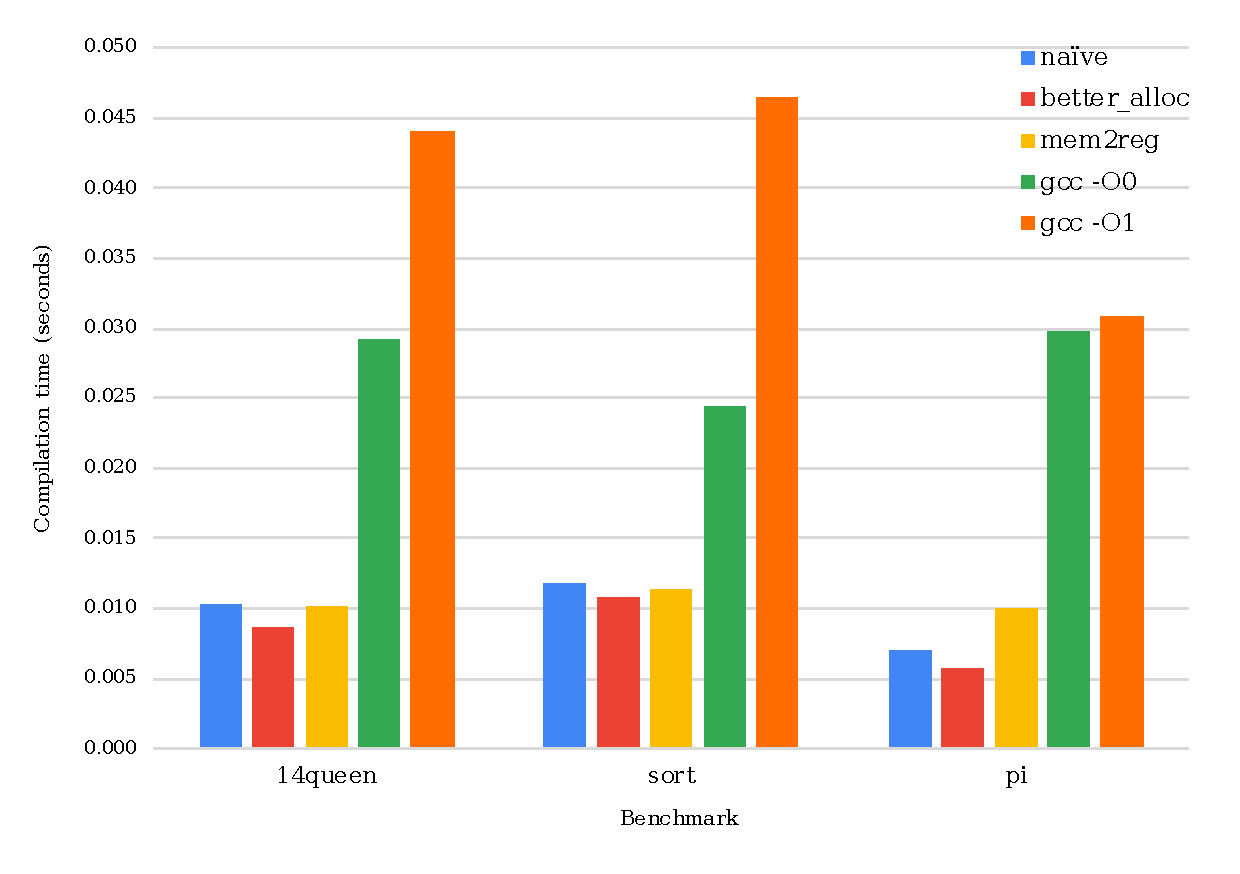
\includegraphics[width=15cm]{graph2.pdf}
  \caption{コンパイラごとのコンパイル時間の比較}
  \label{ccc_bench_compile_graph}
\end{figure}

\clearpage
\paragraph{実行時間}

実行時間のベンチマーク結果を\cref{ccc_bench_run}と\cref{ccc_bench_run_graph}に示す。なお、naiveのsortについてはその時点でのcccの実装にバグがあり実行時エラーが生じているため正常な計測ができていない。

\begin{table}[h]
  \centering
  \begin{tabular}{l|rl|rl|rl|rl|rl}
    &\multicolumn{10}{c}{実行時間, 秒 (gcc -O0との比)} \\ \hline
    &\multicolumn{2}{c|}{naive}&\multicolumn{2}{c|}{better\_alloc}&\multicolumn{2}{c|}{mem2reg}&\multicolumn{2}{c|}{gcc -O0}&\multicolumn{2}{c}{gcc -O1} \\ \hline\hline
    14queen&24.4&(2.27)&25.9&(2.41)&22.7&(2.11)&10.8&(1.00)&5.59&(0.52) \\
    sort&0.30&(0.04)&12.2&(1.55)&11.2&(1.43)&7.86&(1.00)&3.65&(0.46) \\
    pi&23.8&(1.26)&18.9&(1.00)&14.3&(0.76)&18.9&(1.00)&0.00&(0.00) \\
  \end{tabular}
  \caption{ベンチマーク結果: 実行時間}
  \label{ccc_bench_run}
\end{table}

\begin{figure}[h]
  \centering
  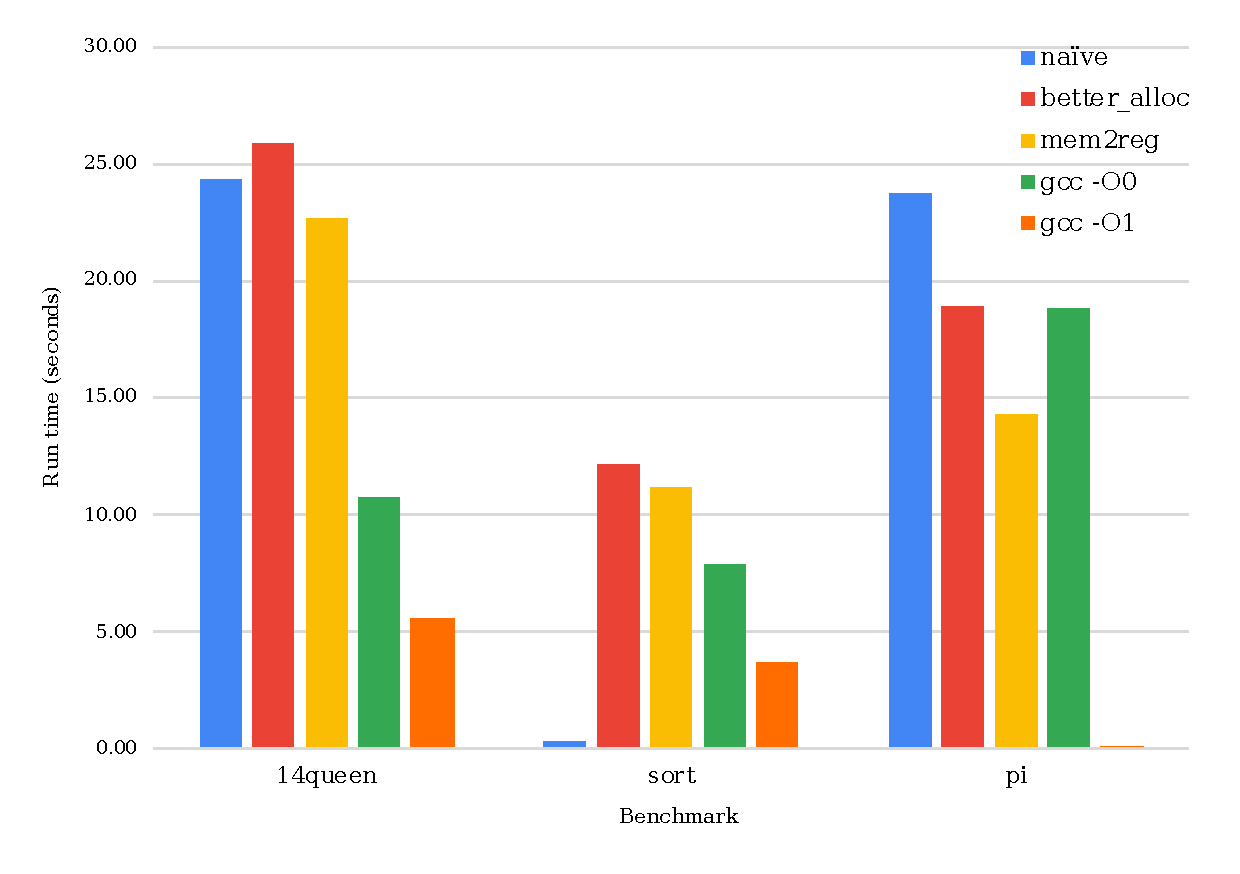
\includegraphics[width=15cm]{graph1.pdf}
  \caption{コンパイラごとの実行時間の比較}
  \label{ccc_bench_run_graph}
\end{figure}

\clearpage
\paragraph{出力コード行数}

出力コード行数のベンチマーク結果を\cref{ccc_bench_loc}に示す。

\begin{table}[h!]
  \centering
  \begin{tabular}{l|rl|rl|rl|rl|rl}
    &\multicolumn{10}{c}{行数 (gcc -O0との比)} \\ \hline
    &\multicolumn{2}{c|}{naive}&\multicolumn{2}{c|}{better\_alloc}&\multicolumn{2}{c|}{mem2reg}&\multicolumn{2}{c|}{gcc -O0}&\multicolumn{2}{c}{gcc -O1} \\ \hline\hline
    14queen&673&(2.50)&656&(2.44)&630&(2.34)&269&(1.00)&250&(0.93) \\
    sort&747&(2.46)&709&(2.33)&655&(2.15)&304&(1.00)&253&(0.83) \\
    pi&234&(2.07)&217&(1.92)&199&(1.78)&113&(1.00)&42&(0.37) \\
  \end{tabular}
  \caption{ベンチマーク結果: 出力コード行数}
  \label{ccc_bench_loc}
\end{table}

\end{document}
